\section{Theorie}
\label{sec:Theorie}

\subsection{Austrittsarbeit und die Energieverteilung der Leitungselektronen}
Metalle sind fast immer kristalline Festkörper, wo die auf den Kristallgitterplätzen sitzenden Atome ausnahmslos ioniesiert sind.
Somit ist ein wesentliches Kennzeichen von Metallen die gute elektrische Leitfähigkeit.
Von den freigesetzten Elektronen wird dieses räumlich periodische Gitter umhüllt.
Dieses, nicht zu einem bestimmten Atom zugehörigen, Elektronen heißen Leistungselektronen.
Das Gitterpotential muss einer periodischen Funktion des Ortes entsprechen, aber ist in grober Näherung als konstant anzunehmen.
Somit hat das Metallinnere ein einheitlich positives Potential, welches um einen Betrag \Phi vom Außenraum verschieden ist.
Es wirken keine Kräfte auf die Elektronen im Inneren.
Sie können sich frei bewegen und somit eine hohe Leitfähigkeit erzeugen.
Wenn ein Elektron jedoch den Verbund verlassen will, dann muss es gegen das Potential \xi anlaufen können (Abb \ref{fig:abb1}).
Es muss die sogenannte Austrittsarbeit $e_0\xi$ leisten können.
\begin{figure}
    \centering
    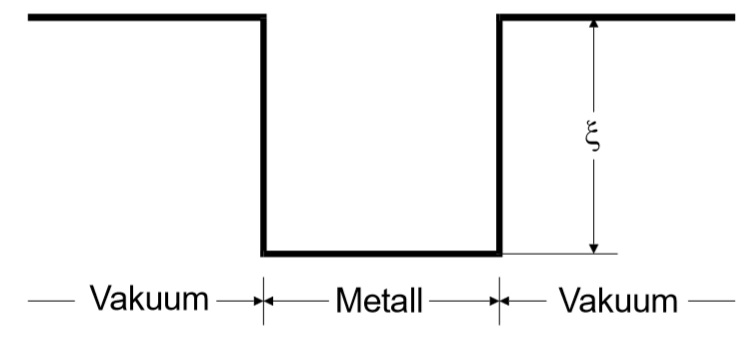
\includegraphics[height=4.0cm]{data/abb1.jpg}
    \caption{Potentialtopf-Modell eines Metalles \cite{V504}}
    \label{fig:abb1}
\end{figure} \\
\noindent
Die Elektronen können nur diskrete, wenn auch sehr dicht beeinander liegende Energiewerte annehmen.
Als Teilchen mit halbzahligem Spin unterliegen die Elektronen eines Kristallgitters dem Pauli-Verbot, das besagt, dass jeder mögliche Zustand mit der Energie E von höchstens 2 Elektronen, die entgegengesetzten Spin haben müssen, eingenommen werden kann.
Das hat zur Konsequenz, dass selbst am absoluten Nullpunkt die Elektronen noch eine endliche Energie besitzen müssen, ganz im Gegensatz zur klassischen Statistik, die jedem Elektron im Mittel die Energie $\frac{3}{2}\text{k}T$ zuordnet.
Die Maximalenergie der Elektronen bei $T = 0$ ist abhängig von der Zahl n der Elektronen pro Volumeneinheit im Metall.
Man bezeichnet sie als Fermische Grenzenergie \xi.
Bei Zimmertemperatur ist für alle Metalle $\xi >> \text{k}T$.
Die Wahrscheinlichkeit dafür, dass im thermischen Gleichgewicht ein möglicher Zustand mit der Energie E besetzt ist, wird durch die Fermi-Diracsche Verteilungs-Funktion angegeben.
Sie hat die Gestalt
\begin{equation}
    \text{f}(\text{E}) = \frac{1}{\text{exp}\left(\frac{\text{E} - \xi}{\text{k}T}\right) + 1}
    \label{eqn:gl1}
\end{equation}
Ein Elektron muss mindestens die Energie $\xi + e_0 \Phi$ besitzen, um die Metalloberfläche zu verlassen, wie man im Verlauf der Gleichung \ref{eqn:gl1} sieht in Abb. \ref{fig:abb2}.
Der Energiewert ist selbst beim Schmelzpunkt von Wolfram noch groß gegnüber $\text{k}T$, sodass die Exponentialfunktion aus Gleichung \ref{eqn:gl1} die Zahl 1 weit übertrifft.
Für Elektronen mit höherer Energie als solche gilt in Näherung
\begin{equation}
    \text{f}(\text{E}) \approx \text{exp}\left(\frac{\xi - \text{E}}{\text{k}T}\right)
    \label{eqn:gl2}
\end{equation}
\begin{figure}
    \centering
    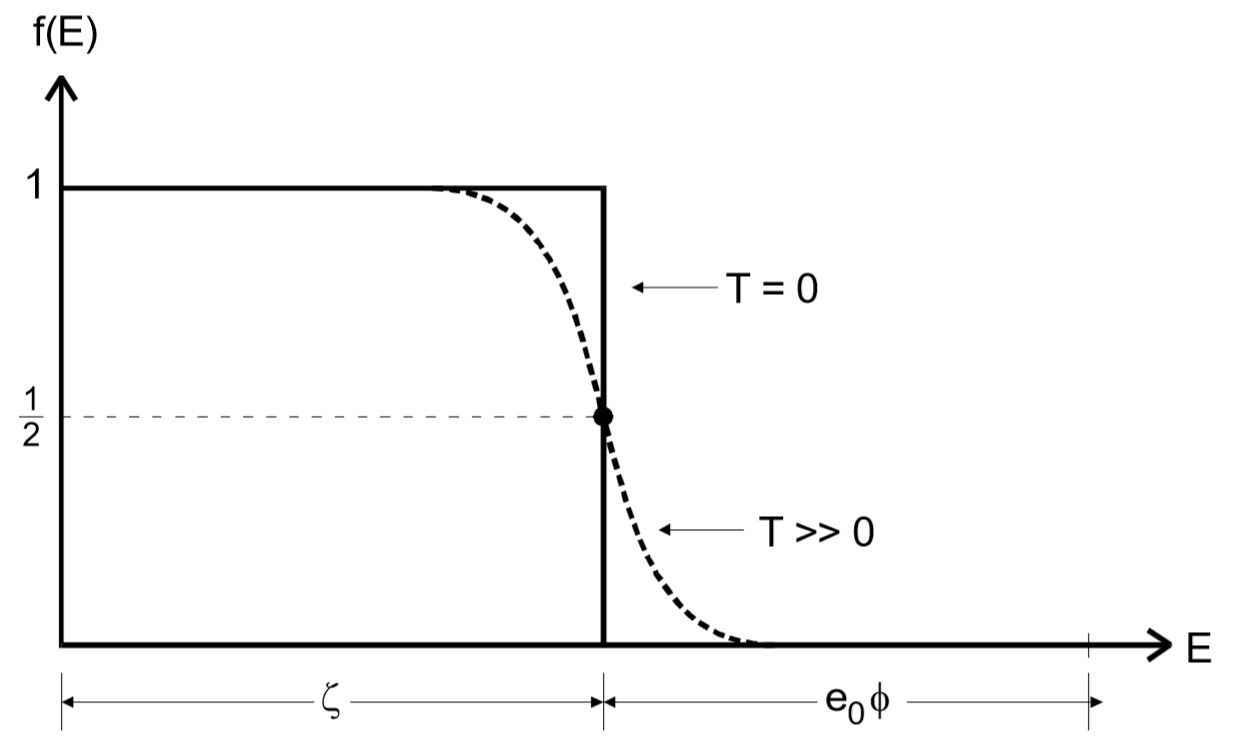
\includegraphics[height=4.0cm]{data/abb2.jpg}
    \caption{Verlauf der Fermi-Diracschen Verteilungsfunktion am absoluten Nullpunkt (durchgezogene Linie) und bei T >> 0 (gestrichelt) \cite{V504}}
    \label{fig:abb2}
\end{figure} \\
\noindent

\subsection{Sättigungsstromdichte}
Aus Gleichung \ref{eqn:gl2} soll die Sättigungsstromdichte $j_s(T)$ in Abhängigkeit von der Temperatur errechnet werden.
Dazu wird ein Koordinatensystem mit Z-Achse senkrecht zur Oberfläche des Metalls eingeführt.
Durch die Zahl der Elektronen aus dem Volumenelement des Impulsraumes und einiger Beziehungen erhält man zuerst die Gleichung
\begin{equation}
    \text{d}\alpha = \frac{\partial \text{E}}{\partial p_z} \text{n}(\text{E}) \text{d}p_x \text{d}p_y \text{d}p_z = \text{n}(\text{E}) \text{d}\text{E} \text{d}p_x \text{d}p_y \text{d}p_z
    \label{eqn:gl3}
\end{equation}
Mit n(E) als Zahl der Elektronen pro Volumeneinheit und d\alpha als die Zahl der Elektronen aus dem Volumenelement des Impulsraumes.
Da jeder Quantenzustand im (sechsdimensionalen) Phasenraum das Volumen $\text{h}^3$ einnimmt, ergibt sich für n(E) der Ausdruck 
\begin{equation}
    \text{n}(\text{E}) = \frac{2}{\text{h}^3}\text{f}(\text{E})
    \label{eqn:gl4}
\end{equation}
Somit können mit Gleichung \ref{eqn:gl3} alle Elektronen die Metalloberfläche verlassen, deren deren Geschwindigkeitskomponente vz so groß ist, dass
\begin{equation}
    \frac{p_z^2}{2\text{m}_0} > \xi + e_0 \Phi
    \label{eqn:gl5}
\end{equation} 
gilt.
Man erhält daher die gesuchte Stromdichte $j_s(T)$ aus Gleichung \ref{eqn:gl3}, indem man alle Elektronen, deren Energiekomponente in Z-Richtung die Ungleichung \ref{eqn:gl5} erfüllt, abzählt und den erhaltenen Zahlenwert mit der Elementarladung $e_0$ multipliziert.
Somit ist 
\begin{equation}
    j_s(T) = 4 \pi \frac{e_0 \text{m}_0 \text{k}^2}{\text{h}^3}T^2 \text{exp}\left(\frac{-e_0 \Phi}{\text{k} T}\right)
    \label{eqn:gl6}
\end{equation}
Die Gleichung \ref{eqn:gl6} wird als Richardson-Gleichung bezeichnet.

\subsection{Die Hohvakuum-Diode}
Die Messung des Sättigungsstromes einer emittierenden Metalloberfläche ist nur im Hochvakuum möglich, da sonst die freien Elektronen in Wechselwirkung mit den Gasmolekülen treten würden.
Sie besteht aus einem evakuierten Glaskörper, mit einer Glühkatode.
Durch einen Strom kann dieser auf eine Temperatur von 1000 bis 3000 K erhitzt werden.
Die aus der Drahtoberfläche austretenden Elektronen werden durch ein elektrisches Feld, das man zwischen der Kathode und einer ihr gegenüberstehenden zweiten Elektrode, der Anode, durch Anlegen einer äußeren Spannung erzeugt, abgesaugt.
\begin{figure}
    \centering
    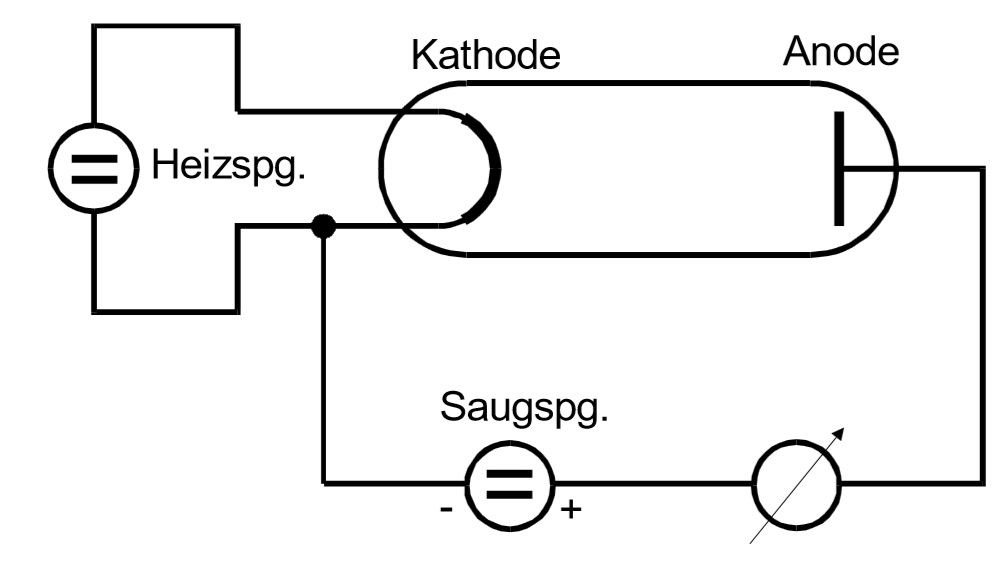
\includegraphics[height=4.0cm]{data/abb3.jpg}
    \caption{Beschaltung einer Hochvakuum-Diode \cite{V504}}
    \label{fig:abb3}
\end{figure} \\
\noindent

\subsection{Die Langmuir-Schottkysche Raumladungsgleichung}